\section{Introduction}
One of the easiest IPS to implement is WLAN IPS. The adaptation of such a system comes without extra cost as most of the hardware is already prevalent in large, indoor environments. 
WLAN is specified by IEEE in their 802.11 specification, determining the WLAN protocols and most widespread operating bandwidth of about 2.4GHz and 5.8GHz \cite{Techopedia} \cite{ElectronicsNotes}\cite{Cisco}. 
\section{Indoor Positioning Topology}
Three topologies exists that can be used for gathering information about the position, as listed below \cite{Henniges2012}:
\begin{enumerate}
\item Network-based topology: position is determined by a central server and different \acrshort{ap}s;
\item Terminal-based: the position is identified by the mobile device;
\item Terminal-assisted: hybrid version of 1. and 2., where 
\end{enumerate}
\begin{figure}[h!]
\centering
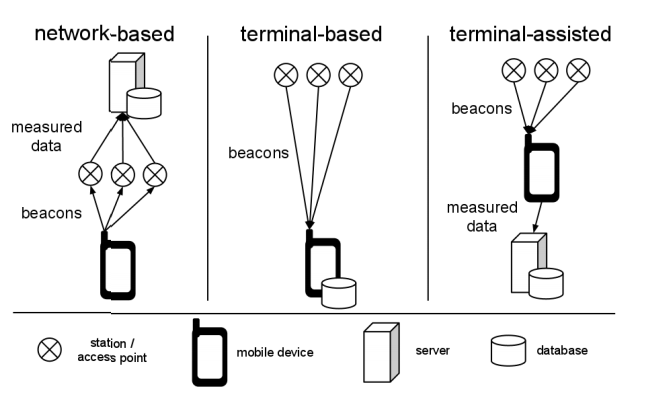
\includegraphics[scale=0.75]{ips_topologies}
\caption{IPS Topologies ~\cite{Henniges2012}}
\label{fig:ips_topologies}
\end{figure}
\subsection{Network-based}
This method only functions when the \acrshort{ap}s are adapted to not only receive network data but also signal data and redirect this to a central server that can handle and compute the data. This requires a change in the software of each \acrlong{ap}.
\subsection{Terminal-Based}
In this specific topology, the device driver of the \acrshort{ap} or terminal broadcasts beacons in its signalling range so a client can determine the best connectivity to a certain \acrshort{ap} and determine which \acrshort{ap} will be used. There are two ways of obtaining this information: active probing and \acrshort{rf} monitoring. The RF monitoring is a form of passive scanning that listens to the periodic broadcasting by the \acrlong{ap}s, this is important to identify a connection in decline (due to significant noise on the signal, also known as \acrfull{snr}) . When using active probing, the driver sends request frames to each known channel to detect any active WLAN connections. Each \acrshort{ap} receiving a request frame will in its turn respond with a response frame. These packets contain the \acrshort{mac} addresses of available devices. Based on this list of available devices and the corresponding signal strength (obtained from services that provide the information via the \acrshort{mac}-layer) an optimal \acrshort{ap} is selected\cite[p.~8]{Retscher}.
\subsection{Terminal-Assisted}
\section{Indoor Positioning Techniques}
The main difficulty in using this technique is determining the position of a device, relative to a Wi-Fi \acrfull{ap}. There are two mainly used technologies to determine the location of a \acrfull{mu}, being: multi- or trilateration and fingerprinting.
\subsection{Trilateration Technique}
Trilateration, or multilateration, is based on a mathematical approach that incorporate the characteristics of the \acrshort{ap} and its signals, such are: characteristics of the radio signal (wavelength, frequency, noise etc.), \acrfull{mac} address of the \acrlong{ap} and the position of WLAN \acrshort{ap}s. This approach requires three base points to calculate and determine a point in range of these three base points. Applying this method to the current case in which the available base points are the \acrshort{ap}s and the \acrshort{mu}, one has to calculate the distance of the \acrlong{mu} to each of the three \acrshort{ap}s in the vicinity. The main difficulty using this method is the estimation of the distances between both the \acrshort{ap}s and the device. Commonly used methods to determine the distance between both the AP as well as the mobile user include: received signal strength, \acrfull{toa} from transmitters or \acrfull{tdoa} \cite[p.~1]{Shchekotov}.
\subsubsection{Geometric Distance Estimation}
The signal propagation model proposed in the previous paragraph indicates the need of an equation system containing three measurements of distance between \acrshort{ap} and \acrlong{mu}. Using the euclidean distance between two points, this results in the following system or model \cite{CutTheKnot}:
\[ \sqrt{(x-x_1)^2 - (y-y_1)^2} = d_1 \]
\[ \sqrt{(x-x_1)^2 - (y-y_1)^2} = d_2 \]
\[ \sqrt{(x-x_1)^2 - (y-y_1)^2} = d_3 \]
By solving this system of equation, each distance is considered to be the radius of a circle, starting at the \acrshort{ap}. The three circles created by according radius contain an intersection point, the specific location of the user, as visualized in figure 4.1.
\begin{figure}[h!]
\centering
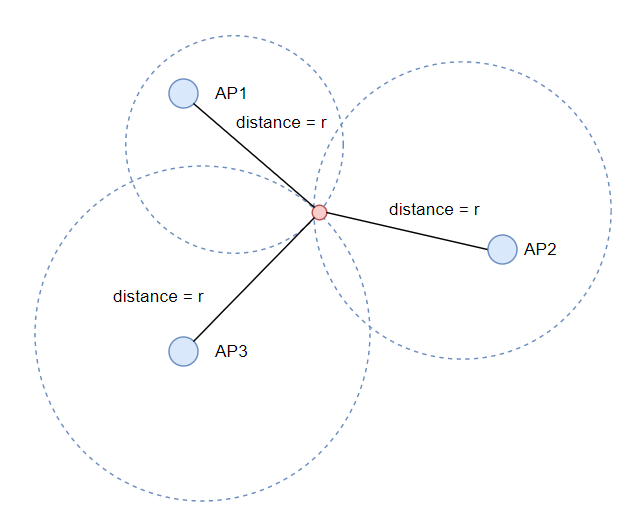
\includegraphics[scale=0.75]{euclidean_distance}
\caption{Euclidean distance resulting in geometric intersection of three circles, determining the position of a point in between these three points.}
\label{fig:euclidean}
\end{figure}
\subsubsection{Based on Signal Propagation Model}
To handle the loss and gain of the radio signal, a free-space path loss model is an optimal solution, as seen in an experiment in \cite[p.178]{Shchekotov}. The formula provided by that specific research is as follows:
\begin{equation}
FPSL = 20log10(d) + 20log10(f) – 27.55
\end{equation}
Where the trans;iutter-receiver separation distance is annotated by the variable d and the frequence in Mhz by f. FPSL indicates the received signal strength path loss in dBm.
\subparagraph{Conclusion}
Based on the research done in \cite{Shchekotov}, the signal propagation model using a free-space path loss approach does not provide an accurate estimation of the user's current position and is therefore discarded as such.
\subsubsection{Based on RSS Measurement Collection}
This method uses an empirical (observational) model, generated by trial runs using different calibration points with different \acrlong{ap}s. As seen in experiment in \cite{Shchekotov}, this experiments results in a table containing different measurements of different distances and the received signal strength in dBm, from transmitter to the receiver. This empirical method results in a usable mathematical formula:
\begin{equation}
\delta = \sqrt{\sigma * t)^2 + A^2}
\end{equation}
In this equation $\delta$ annotates the observational error in dBm, $\sigma$ is the standard deviation of the experiment, $t$ is the function of the t-distribution and $A$ is the observational error of the mobile device used in the experiment.
\begin{figure}[h!]
\centering
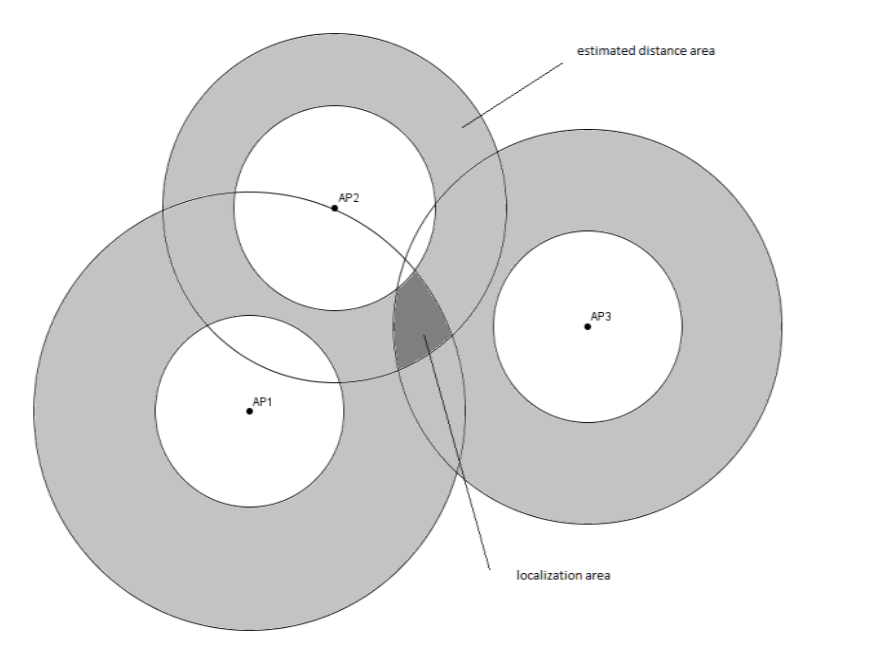
\includegraphics[scale=0.5]{estimated_distance_segments}
\caption{Estimated distance segments ~\cite[p.179]{Shchekotov}}
\label{fig:euclidean}
\end{figure}
\subparagraph{Conclusion}
As seen in the trials performed in the research of \cite{Shchekotov}, this approach can be perceived as a special case of fingerprinting due to the creation of a RSS to AP table. This method results in a more accurate estimation of the user's location by taking the error and deviation into account. However, this research was not based on extensive measurements and it is uncertain this approach will yield an optimal accuracy and precision.
\subsection{Fingerprinting Technique}
A computationally effective method of determining a user's location is the fingerprinting technique. This technique consists of two phases: offline acquisition of \acrshort{rssi} values at particular locations and an online phase with the actual implementation of periodically sent signals from a \acrshort{mu} \cite[p.~9]{Retscher}.
\subparagraph{Conclusion}
This method requires a lot of time to set up the radiomap in the offline phase, but results in a satisfactory accuracy and precision. This is by far the preferred method of providing indoor location using a \acrshort{wlan}-based technology.
\subsubsection{Offline Acquisition}
\subsubsection{Online Phase}
\section{Feasibility}
\subsection{Security and Privacy}
\subsection{Cost}
\subsection{Performance}
\subsection{Robustness and Fault Tolerance}
\subsection{Complexity}
\subsection{Application Use}
\subsection{Commercial Availability}
\subsection{Limitations}

\subsection{Radio Signal}
\section{Conclusion}
